\documentclass[preview]{standalone}

\usepackage{amsmath}
\usepackage{amssymb}
\usepackage{bettelini}
\usepackage{stellar}
\usepackage{definitions}
\usepackage{tikz}
\usepackage{fancybox}
\usepackage{makecell}

\begin{document}

\id{chimica-classificazione}
\genpage

\section{Suddivisione della materia}

\begin{snippetdefinition}{sostanza-pura-elementare}{Sostanza pura elementare}
    Una \textit{sostanza pura elementare} è composta da un solo tipo di elemento.
\end{snippetdefinition}

\begin{snippetdefinition}{sostanza-pura-composta-definition}{Sostanza pura composta}
    Una \textit{sostanza pura composta} è composta da un solo tipo di composto.
\end{snippetdefinition}

\begin{snippetdefinition}{soluzione-definition}{Soluzione}
    Una \textit{soluzione} è una sostanza composta da diversi tipi di composti
    in maniera omogenea.
    Nelle soluzioni viene denominato \textit{solvente} il
    componente presente in maggior quantità e \textit{soluto}
    qualsiasi altra sostanza.
\end{snippetdefinition}

\begin{snippetexample}{sostanza-pura-composta-example}{Sostanza pura composta}
    Acqua (\(H_2O\))
\end{snippetexample}

\begin{snippetexample}{sostanza-pura-elementare-example}{Sostanza pura elementare}
    Azoto (\(N\))
\end{snippetexample}

\begin{snippetexample}{soluzione-example}{Soluzione}
    \(50\% N + 50\% H_2\)
\end{snippetexample}

\begin{snippet}{classificazione-sostanze-miscugli-illustrazione}
\begin{center}
    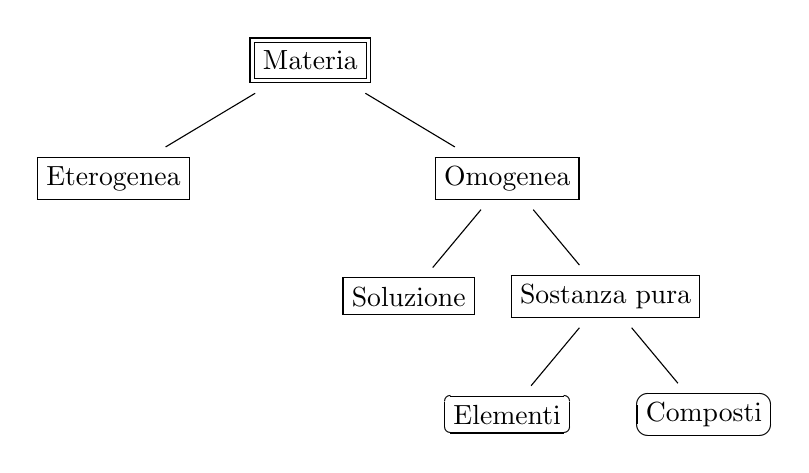
\begin{tikzpicture}[
        level 1/.style = {sibling distance = 5cm},
        level 2/.style = {sibling distance = 2.5cm}
    ]
    \node {\doublebox{Materia}}
        child {
            node {\fbox{Eterogenea}}
        }
        child {
            node {\fbox{Omogenea}}
            child {
                node {\fbox{Soluzione}}
            }
            child {
                node {\fbox{Sostanza pura}}
                child {
                    node {\ovalbox{Elementi}}
                }
                child {
                    node {\ovalbox{Composti}}
                }
            }
        };
    \end{tikzpicture}
\end{center}

\begin{itemize}
    \item La materia può essere classificata come materia \textit{eterogenea}
    e materia \textit{omogenea}.
    
    \item La materia omogenea può essere classificata come \textit{miscuglio omogeneo} (soluzione)
    oppure come \textit{sostanza pura}.
    
    \item Le sostanze pure possono essere classificati come \textit{elementi} oppure \textit{composti}.
\end{itemize}
\end{snippet}

\section{Stati di aggregazione}

\begin{snippet}{stati-aggregazione-expl}
    Gli stati di aggregazione della materia sono gli stati che convenzionalmente può assumere la
    materia a seconda delle sue proprietà meccaniche.\\
    Gli stati che la materia può assumere sono:
    \begin{enumerate}
        \item \textbf{solido}: La materia ha un volume e una forma propria;
        \item \textbf{liquido}: La materia ha un volume proprio, ma acquisisce la forma del
            recipiente che la contiene;
        \item \textbf{gassoso}: La materia non ha né volume né forma propria, ma si espande fino
            a occupare tutto lo spazio disponibile;
        \item \textbf{plasmatico}:
        La materia ionizzata non ha né volume né forma propria, ma si espande fino
        a occupare tutto lo spazio disponibile;
    \end{enumerate}
\end{snippet}

\section{Transizione di fase}

\begin{snippet}{tranizioni-di-fase-expl}
    La transizione di fase, o passaggio di stato, indica la trasformazione di un sistema termodinamico da uno stato di
    aggregazione ad un altro. Durante questa trasformazione, si registra una variazione dell'entalpia, che quantifica
    il calore scambiato con l'ambiente a seguito del cambiamento di stato.
\end{snippet}

\includesnpt[src=/snippet/static/matter-phases.png|width=100\%]{centered-img}

\end{document}